\documentclass[10pt]{beamer}
\usepackage{xeCJK}
\usepackage{graphicx}
\usepackage{booktabs}
\usepackage{listings}
\usepackage{multirow}
\usepackage{mathtools}
\usepackage{ulem}
\usetheme{metropolis}
\begin{document}
	\title{简单的枚举贪心选讲}
	\date{\today}
	\author{huhao}
	\maketitle
	\clearpage
	\begin{frame}
		\frametitle{前言}
		\onslide<1-> 由于没有什么题目主要是考枚举,所以不怎么讲枚举

		\onslide<2-> 由于贪心比较简单的题没什么意思,也不存在有什么算法不会之类的问题,所以今天的题都不是特别难度

		\onslide<3-> \sout{晚上有CF,所以题目较少}
	\end{frame}
	\clearpage
	\begin{frame}
		\frametitle{贪心基础}

		\onslide<1-1> 贪心主要应用在\sout{猜结论}为最优性问题提供策略上,主要体现在:

		\onslide<2-3> 两种决策,其中$A$的贡献不比$B$小,那么选$B$之前要选$A$

		\onslide<3-3> 如果两种操作$AB$间相互影响,那么需要选$A$后需要添加选$B$然后撤回$A$的操作

		\onslide<4-4> 如果部分操作一定会连续进行,可以尝试合并

		\onslide<5-5> 对于部分题目是若干操作序列让你排列后依次贡献,可以考虑邻项交换

		\onslide<6-6> 如果上面不好想的话,可以尝试先建出费用流,然后利用这张图的特殊性,用较低复杂度模拟出费用流(具体看后面)
	\end{frame}
	\clearpage
	\begin{frame}
		\frametitle{Usaco2015 dec High Card Low Card}
		\par 给定两个数组$a,b$,你需要选择时间$t$并重排列$a$
		\par 在前$t$轮中$a_i>b_i$则产生$1$的贡献,之后$a_i<b_i$则产生$1$的贡献
		\par 求最大贡献
	\end{frame}
	\clearpage
	\begin{frame}
		\frametitle{solution}

		\onslide<1-> 记$f_i$为$t\ge i$时前$i$轮最多产生的贡献,$g_i$为$t<i$时$i$轮及以后产生的最大贡献

		\onslide<2-> 显然要贴着边界去选,然后找$t$让$f_t+g_{t+1}$最大

		\onslide<3-> 如果一个数$x$选了两次,那么至少有一个数$y$没有被选,若$y>x$,那么在把$t$之前的$x$换为$y$不会劣,$y<x$同理
	\end{frame}
	\clearpage
	\begin{frame}
		\frametitle{种树}
		\par 有一个长度为$n$的环,每个点有权值,选择$m$个两两不相邻的点且权值和最大。
		\par 求这最大的权值
	\end{frame}
	\clearpage
	\begin{frame}
		\frametitle{solution}
		\onslide<1-> 考虑到每次要么选一个周围没被选过的点,要么一段区间向外扩展一段

		\onslide<2-> 相当于选一个点$a_i$后把$a_{i-1},a_i,a_{i+1}$缩为$a_{i-1}+a_{i+1}-a_i$

		\onslide<3-> 维护最大值即可
	\end{frame}
	\clearpage
	\begin{frame}
		\frametitle{POI2008 MAF-Mafia}
		\par 给定$n$个神枪手,每个神枪手瞄准一个人,以一定顺序开枪,问最少和最多死多少人
	\end{frame}
	\clearpage
	\begin{frame}
		\frametitle{solution}
		\onslide<1-> 显然,这是一个基环树森林

		\onslide<2-> 对于一个联通块
		
		\onslide<2-> 一个自环:答案始终是$1$

		\onslide<2-> 一个大小为$a$的环:答案$\lfloor\dfrac a2\rfloor\sim a-1$

		\onslide<2-> 一个不只有环的基环树:最大是只剩入度为$0$的,最小是入度为$0$的依次开枪,直到没有没开过枪的活人或剩一个环
	\end{frame}
	\clearpage
	\begin{frame}
		\frametitle{NOI2019序列}
		\par 给定序列$A,B$它们长度为$n$,在这两个序列中各选$m$个数,需要满足至少有$k$个下标$A,B$都选了,求这$2m$个数的最大的和
		\par $k\le m\le n\le 2\times 10^5$
	\end{frame}
	\clearpage
	\begin{frame}
		\frametitle{solution}
		\onslide<1-> 考虑到贪心时决策间有影响,可能需要撤回操作,考虑费用流建图

		\onslide<2-> $A,B$分别向$S,T$连边,边权为权值取相反数,然后相同标号的$A$向$B$连边

		\onslide<3-> 因为有至多$m-k$对不用选相同下标,新建两个点$u,v$,连流量$m-k$费用$0$的边,$A$的点向$u$连,$v$向$B$的点连,就处理掉了$m-k$个可以下标不相同的点了

		\onslide<4-> 要快速模拟出来就只要维护$A$中选了/任意中$B$最大的,$B$中选了/任意中的$A$最大的,$AB$都没选的最大的$A+B$
	\end{frame}
	\clearpage
	\begin{frame}
		\frametitle{CF1208G Polygons}
		\par 给定$n,k$
		\par 你需要构造$k$个有相同外接圆的多边形,使得边数在$3\sim n$间且边数两两不同
		\par 你可以任意旋转它们,求它们与这个外接圆的最少交点数
		\par 下面是$n=6,k=2$(边数为$3,6$)的一种方案
		\par 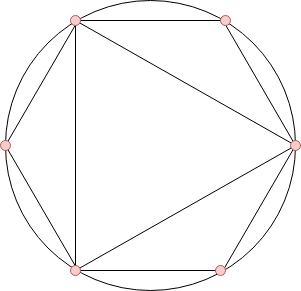
\includegraphics[width = 0.4\textwidth]{1.png}
		\par $k\le n-2,n\le 10^6$
	\end{frame}
	\clearpage
	\begin{frame}
		\frametitle{solution}
		\onslide<1-> 显然,这些多边形会有一个共同的交点

		\onslide<2-> 于是,发现如果$u|v$,那么$u$肯定比$v$先选

		\onslide<3-> 并且如果所有$u|v$都选了,那么$v$的代价为$\phi(v)$

		\onslide<4-> 按$\phi$排序后从小到大选即可,当然因为没有$2$边形,特判掉即可
	\end{frame}
	\clearpage
	\begin{frame}
		\frametitle{IOI2019排列鞋子}
		\par 给定长度为$2n$的数组$S$
		\par 一个数组合法当且仅当$\forall i,\exists j>0,a_{2i-1}=-j,a_{2i}=j$
		\par 每次可以交换相邻两个数,求最少交换次数
		\par $n\le 10^5,1\le |a_i|\le n$
	\end{frame}
	\clearpage
	\begin{frame}
		\frametitle{solution}
		\onslide<1-> 做$n$次,每次把与当前序列中第一个配对的移到前面来(有相同值就取第一个),然后删除

		\onslide<2-> 考虑证明

		\onslide<2-> 显然,当$S_i$有相同的时候,贪心从前往后配对(并给新标号)是对的,记$p_v$为$v$的位置

		\onslide<3-> 把$i$和$−i$配对,要交换$|p_i−p_{−i}|−[p_{−i}<p_i]$次,然后在交换的过程中,对所有$j$,且$p_j$和$p_{−j}$仅有一个在$p_i$到$p_{−i}$区间内,那么它们距离减一

		\onslide<4-> 于是我们从前往后配对即可,把这个过程模拟出来就是上面做法了 
	\end{frame}
	\clearpage
	\begin{frame}
		\frametitle{HNOI2010取石子游戏}
		\par 总共有$n$堆石子依次排成一行,第$i$堆石子有$a_i$个石子。
		\par 部分堆为$0$,如果一堆旁边有石子数为$0$的堆,就可以全部取走
		\par 两人以此操作,问他们都用最优操作时,各能取几个石头
		\par $n\le 10^6$
	\end{frame}
	\clearpage
	\begin{frame}
		\frametitle{solution}
		\onslide<1-> 首先,如果存在$a,b,c$相邻,且$b\ge a,b\ge c$,当先手取了$a$时,接下来的操作一定是:$a\rightarrow b\rightarrow c$($c$同理)

		\onslide<2-> 因为取a一定是非正贡献,先手只能选a,就说明当前最优已经非正了,后手取b一定不劣

		\onslide<2-> 然后如果先手不选c,那么a相当于白选,肯定不优

		\onslide<2-> 于是我们可以把这样的a,b,c合并为a+c−b

		\onslide<3-> 合并完后一定是连续上升或连续下降,除开头外显然从大到小选不劣

		\onslide<3-> 开头的和连续下降末尾的连续上升如果是偶数长度先手就一定不会先选,否则可以纳入从大到小的选择里面

	\end{frame}
	\clearpage
	\begin{frame}
		\frametitle{皇后游戏}
		\par 给定长为$n$的序列$a,b$,对于一个排列$p$,有:
		$$
		f_i=\begin{cases}a_{p_1}+b_{p_1}&i=1\\\max(\sum_{j\le i} a_{p_j},f_{i-1})+b_{p_i}&i\not =1\end{cases}
		$$
		\par 求$f_n$的最小值
	\end{frame}
	\clearpage
	\begin{frame}
		\frametitle{solution}
		\onslide<1-> 我们相邻两项$a_1,b_1,a_2,b_2$,即前面和为$s$上一个$f$值为$F$,显然之后后面那项的$f$对答案有影响,我们要使:

		\onslide<2-> $$
		\begin{aligned}
			\max(s+a_1+a_2+b_2,s+a_1+b_1+b_2,F+b_1+b_2)&\le\\
			\max(s+a_2+a_1+b_1,s+a_2+b_2+b_1,F+b_2+b_1)&
		\end{aligned}
		$$

		\onslide<3-> 可以推出需要满足的条件为$\min(a_i,b_j)<\min(a_j,b_i)$,相等时按$a_i$从小到大排序即可
		
	\end{frame}
	\clearpage
	\begin{frame}
		\frametitle{end}
		\onslide<1-> 本次讲课作为一道noip难度的讲课

		\onslide<2-> 覆盖面广

		\onslide<3-> 难度适中

		\onslide<4-> 题量适中

		\onslide<5-> 解法自然

		\onslide<6-> 讲课人相信,这次美妙的讲课,可以给即将AK[CSP2019|HNOI2020|NOI2020|WC2021|CTS2021|IOI2021]的你,提供一个有力的帮助
	\end{frame}
	\clearpage
	\begin{frame}
		\frametitle{end}
		\begin{center}
			\Huge Thanks for listening
		\end{center}
	\end{frame}
\end{document}